\chapter{Caso de Estudo}

Um dos objetivos desta dissertação passa por demonstrar a capacidade da arquitetura estruturada e implementada em recolher e processar informação através da utilização de diversos tipos de sensores e apresentar resultados com origem nesses dados. Com esse intuito foi feito um caso de estudo sob diversas variáveis com o intuito de demonstrar a funcionalidade da arquitetura. Para tal foi definido um conjunto de sensores a utilizar, de forma a que da monitorização efetuada resultasse informação diversificada, foi também selecionado o tipo de ambientes e situações de monitorização, para além do tipo de utilizadores utilizado neste caso de estudo. Foram ainda utilizadas os serviços de métricas integrados na arquitetura relacionados com os tipos de dados recolhidos, de forma a processar a informação e alcançar um diferente nível de dados. Tudo isto permitiu alcançar um conjunto de resultados que será apresentado neste capítulo, bem como todo os passos percorridos até alcançar esses resultados.


\section{Sensores Utilizados}

A escolha dos sensores a utilizar neste caso de estudo tiveram por base várias razões e condicionantes de acordo com o objetivo a alcançar com esta demonstração em particular. Tendo então como principal intuito demonstrar a funcionalidade e capacidade de recolha, comunicação entre os diversos componentes e processamento da informação, os sensores escolhidos tiveram, para além do acesso a este tipo de dispositivos, como base a diversidade dos dados, a fiabilidade dos equipamentos, o comportamento dos utilizadores a monitorizar e ainda os serviços de métricas previamente integrados na arquitetura. Foi sob este fatores que foi selecionado um conjunto de sensores que se pretende que cumpram os requisitos definidos.

Com base neste conjunto de fatores e tendo em conta a importância de cada um foram selecionados três tipos de sensores para esta demonstração: rato, teclado e acelerómetro. Estes três tipos de sensores, em primeiro lugar, são sensores aos quais era possível facilmente aceder e de simples utilização para os seus utilizadores. Este tipo de equipamento são equipamentos muito utilizados em diversos contextos e há bastante tempo. Isto confere-lhe um nível de segurança e de desenvolvimento tecnológico (citação) que garante um pressuposto fundamental nesta escolha que diz respeito à fiabilidade do equipamento e da informação recolhida. O facto deste conjunto de sensores escolhido ser composto por três tipos de sensores, corresponde a um número aceitável de opções dado que levará a um número de serviços de métricas a utilizar mais alargado e garante um nível de diversidade de informação suficiente para demonstrar a funcionalidade e capacidade de recolha da arquitetura desenvolvida.

Outro fator fundamental na seleção deste três tipos de sensores prende-se com o comportamento e contexto de monitorização por parte dos diferentes utilizadores neste caso de estudo. Esta demonstração pretende, como base de recolha de informação, extrair do comportamento dos seus utilizadores a forma como estes interagem com o computador, como ferramenta de trabalho ou noutro qualquer contexto fora deste âmbito, bem como registar alterações de comportamentos derivados da ocorrência de estados como, por exemplo, o stress. Com base neste objetivo, a utilização deste três tipos de sensores enquadra-se perfeitamente dado que incidem sobre os dispositivos mais comuns usados pelos utilizadores para interagir com a máquina. Consequentemente, é também através destes que a sua iteração e os seus comportamentos evidenciarão alterações de comportamento ao longo do tempo (citação). 

O conjunto de fatores e correspondentes decisões tomadas que levaram à escolha da seleção de sensores apresentada garantem os pressupostos necessários para cumprir os objetivos pretendidos com este caso de estudo. Desta forma será possível alcançar resultados que demonstrem a funcionalidade da arquitetura e sua utilidade para os seus utilizadores.



\section{Tipos de Utilizadores(rever - alterar dados os resultados)}

Na construção de um caso de estudo, como método de demonstrar a funcionalidade e utilidade da arquitetura desenvolvida neste caso em particular, existem várias questões que devem ser ponderadas. Uma delas consiste no perfil de utilizadores escolhidos para a demonstração e na sua diversidade. Deste modo, importa garantir que o conjunto de utilizadores escolhidos para a recolha de dados através da utilização da arquitetura apresentam diferentes características com o intuito de acrescentar solidez aos resultados finais e assim conseguir retirar conclusões mais fiáveis.

Com base neste pressuposto, foram ponderadas todas as características da arquitetura apresentadas para definir um conjunto de utilizadores adequado ao objetivo deste caso de estudo. Posto isto, foi definido um conjunto de três utilizadores com diferentes faxas etárias, diferentes interesses, bem como diferentes características pessoais e personalidades diferentes. Com esta opção pretende-se aumentar a probabilidade de verificar resultados diversificados para os vários parâmetros a analisar, com recurso ao mesmo tipo de aparelhos de monitorização.

Foram então escolhidos três pessoas para testar a arquitetura através da utilização dos três tipos de sensores apresentados. Dois utilizadores têm 24 anos e outro tem 32 anos. Todos eles são pessoas ligadas à área da informática, estando a sua vida profissional diretamente ligada à utilização de computadores, sendo assim possível recolher informação sobre todos em diversos contextos de utilização. Todos eles têm personalidades distintas, um é uma pessoa extremamente calma e ponderada, outro um trabalhador incansável que passa imenso tempo a trabalhar, e o terceiro trata-se de uma pessoa bastante impulsiva e stressada. A diversidade de personalidades e perfil das pessoas escolhidas aliadas à possibilidade de todos serem monitorizados em diferentes ambientes mas que lhes são naturais e familiares permitem a diversidade de condicionantes pretendida para este caso de estudo.


\section{Ambientes de teste}

Depois de definidos os tipos de utilizadores e meios tecnológicos para construir o caso de estudo, falta analisar quais os tipos de contextos mais adequados para efetuar a recolha de informação. A definição destes contextos deve ter em conta que, naturalmente, existem situações cuja tendência a ocorrer determinados tipos de reação é mais propícia do que noutras. Por exemplo, no caso da monitorização ocorrer num ambiente de trabalho, a tendência a verificar-se indicadores de stress ou fadiga com o passar do tempo é bastante mais provável do que verificar-se esses indícios em situações de lazer ou divertimento.

Posto isto, deve ser definido um conjunto de momentos e contextos durante os quais os utilizadores selecionados devem, de forma menos intrusiva possível, ser monitorizados. Pretende-se desta forma também garantir que a utilização de sensores para recolher informação não interfiram com o normal comportamento das utilizadores, independentemente do ambiente em que este se encontra no momento. Sendo que os sensores definidos para este caso em particular garantem esse requisito. Para além disso, os ambientes de teste definido deve ser igual para todos os utilizadores e deve ser ainda diversificado. Ou seja, todos os utilizadores devem ser sujeitos aos mesmos tipo de ambientes e às mesmas condições de modo a que seja possível comparar os diferentes resultados entre estes. Deve também ser definido um conjunto de ambientes amplo de modo
a que situações distintas possam ser analisadas e comparados resultados entre ambientes em que as diferenças sejam acentuadas.

Tendo em conta a relevância de todos os pontos já descritos foram escolhidas três situações para a recolha de informação neste caso de estudo. A primeira situação escolhida foi o ambiente de trabalho, em que os utilizadores, todos eles sujeitos à utilização do computador no seu período de trabalho, estão constantemente a ser monitorizados durante largos períodos de tempo. Esta situação é muito específica pois tratam-se de ambientes normalmente intensos, desgastantes e por vezes de grande stress para os utilizadores, sendo provável a ocorrência de comportamentos que revelem indicações nesse sentido. A segunda situação definida foi a utilização livre da Internet, ou seja, trata-se de um ambiente fora do âmbito de trabalho em que o utilizador navega normalmente na Internet de forma livre. Trata-se portanto de uma situação de lazer e descanso para o utilizador. O terceiro e último ambiente de utilização definido foi a utilização do Facebook, dado que é uma rede social de ampla utilização atualmente, em que todos os utilizadores se sentem familiarizados e em que normalmente passam muito do seu tempo diariamente. A utilização do Facebook está diretamente relacionada com vários aspetos emocionais e pessoais da vida das pessoas, dada a forma como as pessoas normalmente a utilizam e envolvem na sua vida. Isto pode originar comportamentos e reações bastante interessantes por parte dos seus utilizadores durante a monitorização.

\begin{figure}[htb]
   \centering
   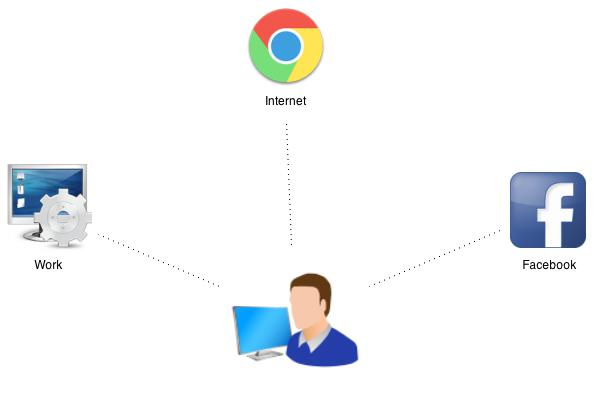
\includegraphics[scale=0.5]{Images/ambientesestudo.jpg}
   \caption{Ambientes de teste definidos}
\end{figure}

\section{Serviços utilizados}

A decisão sobre que serviços a utilizar neste caso de estudo foi essencialmente baseada nos sensores utilizados e consequentemente no tipo de dados recolhidos. Depois de fundamentadamente terem sido escolhidos um conjunto de sensores para esta experiência, os serviços de métricas responsáveis pelo processamento da informação recolhida deverão corresponder logicamente ao tipo de dados correspondente. Os serviços usados deverão ser ainda, dentro deste parâmetro, o mais abrangente possível, ou seja, utilizar o máximo de métricas possíveis, de modo a maximizar a diversidade de informação deste nível de refinamento.

Com base nestes parâmetros, os serviços utilizados neste caso em particular foram os correspondentes aos três tipos de dados levantados: rato, teclado e acelerómetro. A estes três tipos de dados correspondem, tal como apresentado no capítulo anterior os seguintes tipos de serviços: ..... Este panóplia de serviços permitem alcançar um conjunto diversificado de indicadores, num nível de informação acima dos dados em bruto e deste modo enriquecer os resultados deste caso de estudo. 

\section{Resultados}

O caso de estudo efetuado teve por base todas as decisões tomadas e explicadas neste capítulo. Isso permitiu definir um conjunto de \textit{guidelines} com o intuito dos resultados do estudo demonstrarem a funcionalidade e utilidade da arquitetura desenvolvida, que é o seu principal objetivo. Pretende-se ainda apresentar diferenças percetíveis entre os resultados de monitorização dos utilizadores nos diversos momentos e ambientes definidos para este caso em particular. Desta forma serão apresentados os resultados alcançados, sublinhando determinados pontos e conclusões mais relevantes dado que o conjunto total de informação recolhido é bastante extenso.

Entre os diversos serviços de métricas integrados na arquitetura e utilizados neste caso de estudo resultaram grandes blocos de informação cujos resultados se revelaram bastante úteis e esclarecedores em diversos aspetos. De forma a analisar os resultados alcançados serão apresentados nesta secção análises comparativas no que diz respeito aos três utilizadores deste caso de estudo nas três tarefas definidas. Os resultados apresentados nesta secção foram selecionados por serem representativos da generalidade dos resultados alcançados, mas também por demonstrarem algumas características que se pretendia provar nesta experimentação.

Posto isto, e tal como já foi apresentado este caso de estudo foi feito por três utilizadores com diferentes características de forma a analisar o seu comportamento em diversos parâmetros na execução de três tarefas diferentes. Uma dessas tarefas corresponde à utilização do Facebook. Neste aspeto o serviço de métricas em particular que revelou resultados mais interessantes foi  o \textit{Key Down Time}. Este serviço de métrica corresponde aos dados recolhidos pelo sensor de teclado e apresenta o tempo durante o qual uma tecla é pressionada. A análise dos dados recolhidos e processados permite concluir que os três utilizadores apresentaram resultados bastante diferentes.

O primeiro utilizador foi o que apresentou resultados mais altos revelando uma média correspondente ao dobro do segundo utilizador e muito superior ao terceiro utilizador. O terceiro utilizador revelou-se, de longe, o que menos tempo pressionava as teclas. Para além disso, a análise gráfica permite concluir que este último foi o mais constante entre os três utilizadores, havendo a registar três períodos no início em que os valores obtidos se distanciaram do habitual. O segundo utilizador apresenta, ainda assim, dados também relativamente constante registando-se apenas seis momentos em que os valores subiram para valores bastante altos. O primeiro utilizador revelou-se o mais instável neste particular, registando-se várias variações durante o período de monitorização. O facto da variação das médias ser tão acentuado prende-se também com a ocorrência de variações pontuais dos registos cuja visualização não é percetível graficamente por se tratarem de situações pontuais e não de períodos em que se verifiquem variações efetivas dos valores obtidos.

\begin{figure}[htb]
   \centering
   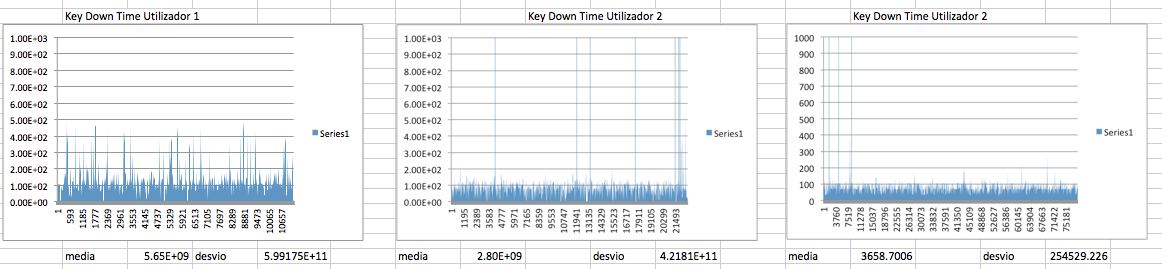
\includegraphics[scale=0.3]{Images/keydowntime.png}
   \caption{Gráficos de resultados de Key Down Time dos três utilizadores na utilização do Facebook}
\end{figure}

A navegação de forma livre por parte dos utilizadores na Internet foi outro dos ambientes de monitorização ao qual estes foram sujeitos. No que diz respeito aos resultados obtidos através dos serviços de métricas importa realçar os resultados do \textit{Time Between Keys}. Esta métrica, também referente aos dados provenientes da utilização do teclado, representa o tempo percorrido entre duas teclas pressionadas. Neste aspeto o primeiro utilizador revelou o comportamento mais tranquilo, tal como indica o seu resultado médio. A análise gráfica dos seus resultados permitem verificar que este se revelou o utilizador com menor número de variações significativas durante o seu período de utilização da Internet, nesta componente em particular. O segundo e terceiro utilizadores já revelaram um elevado número de variações acentuadas no que ao seu comportamento diz respeito. Para além tiveram médias de tempo percorrido entre duas teclas pressionadas superiores, especialmente o segundo utilizador, apresentando já uma diferença significativa para o primeiro utilizador.

\begin{figure}[htb]
   \centering
   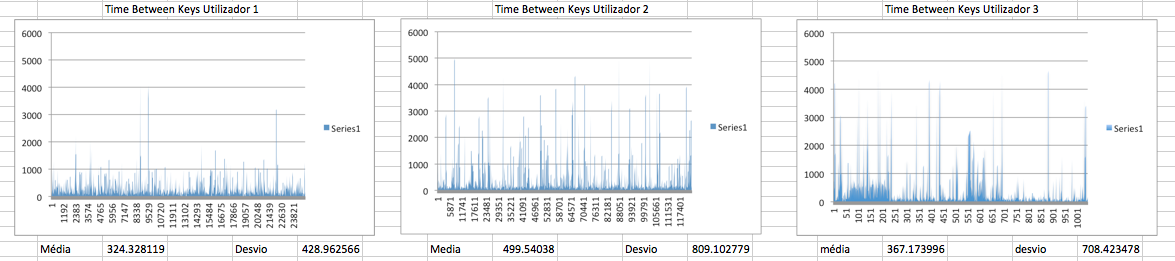
\includegraphics[scale=0.3]{Images/timebetweenkeys.png}
   \caption{Gráficos de resultados de Time Between Keys dos três utilizadores na utilização da Internet}
\end{figure}

Estes resultados indicam uma escrita mais rápida por parte do primeiro utilizador e no sentido oposto uma escrita menos constante mas mais pausada por parte do segundo utilizador. Para além disso, sublinhar que este contexto de monitorização é o contexto escolhido menos condicionante para o utilizador da arquitetura neste caso de estudo.

O outro contexto de monitorização definido foi o período de trabalho dos utilizadores. Este contexto normalmente é o mais intenso e desgastante dos três. De forma a poder comparar o desempenho dos três utilizadores neste ambiente são apresentados o resultados dos utilizadores correspondentes à velocidade do rato durante este período. Neste caso, os valores apresentados demonstram um cenário praticamente oposto aos resultados de monitorização apresentados para a utilização da Internet.

Os resultados do segundo utilizador demonstram que este foi o mais calmo, relativamente ao movimento do rato, durante o seu período de trabalho, registando-se também variações menos acentuados nos seus registos relativamente aos restantes utilizadores. O terceiro utilizador teve resultados próximos do segundo, revelando apenas um ligeiro aumento na sua média, tendo algumas variações mais acentuadas mas ainda assim um desvio padrão inferior ao segundo utilizador. Por fim, o primeiro utilizador foi o mais que apresentou resultados mais elevados, o que indica maior intensidade no seu período de trabalha comparativamente com os restantes utilizadores. A média de resultados apresentada pelo primeiro utilizador é superior aos restantes, bem como o seu desvio padrão e valores alcançados em determinados registos. De salientar ainda que este utilizador trata-se do utilizador indicado neste capítulo como uma pessoa extremamente trabalhadora.

 \begin{figure}[htb]
   \centering
   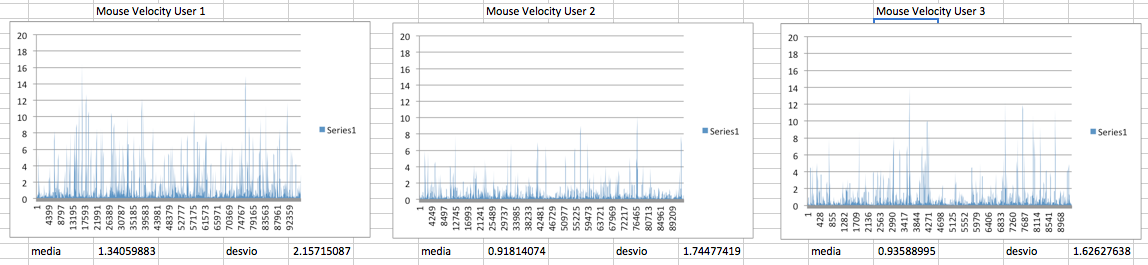
\includegraphics[scale=0.3]{Images/mousevelocity.png}
   \caption{Gráficos de resultados de Mouse Velocity dos três utilizadores durante o período de trabalho}
\end{figure}

Outra análise relevante que deve ser tido em conta é a comparação de resultados obtidos pelo mesmo utilizador na execução de diferentes tarefas. Esta comparação permitirá verificar a diferença de comportamento de um utilizador sob condições diferentes e retirar conclusões sobre esses factos. Posto isto, foram selecionados os resultados do segundo utilizador para a métrica de \textit{Absolute Sum of Angles} que permite quantificar o desvio do movimento do rato independentemente da sua direção. Os resultados desta métrica, teoricamente, terá tendência a apresentar valores mais altos em situações de maior desgaste ou stress, por exemplo.

Os resultados obtidos desta forma apresentam diferenças significativas entre a monitorização efectuada durante a utilização do Facebook e Internet em relação à monitorização durante o período de trabalho. Os valores obtidos durante os dois primeiros contextos apresentam valores bastante semelhantes, tanto para os valores médios e desvios padrões como até graficamente é visível. Esta semelhança de valores indica que em ambas as situações o segundo utilizador teve comportamentos semelhantes neste parâmetro em particular. Já no que diz respeito ao período de trabalho as diferenças são bastante acentuadas. A média e desvio são bastante superiores, sendo até necessário utilizar uma escala bastante maior para fazer a representação gráfica destes valores. 

 \begin{figure}[htb]
   \centering
   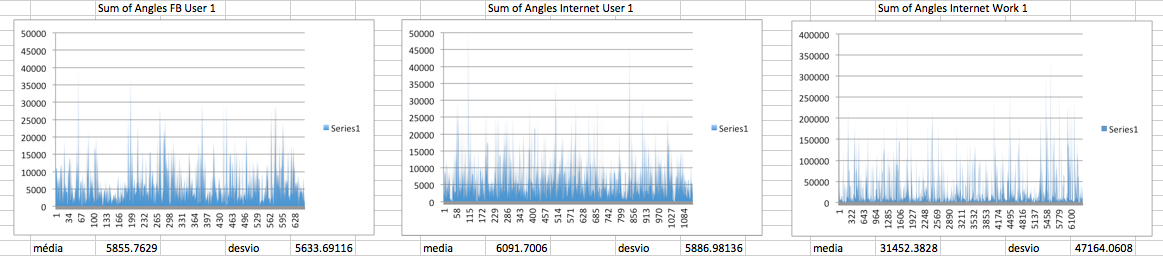
\includegraphics[scale=0.3]{Images/sumofangles.png}
   \caption{Gráficos de resultados de Absolute Sum of Angles das três tarefas realizados pelo segundo utilizador}
\end{figure}

Estes valores demonstram de facto uma diferença acentuada entre duas situações de lazer, navegar na Internet e utilização de Facebook, relativamente a uma situação de trabalho com toda a carga que este contexto implica. O facto de ser um contexto mais pesado e com maior probabilidade de existência de situações como a fadiga e stress, justifica a variação de resultados entre os contextos analisados neste caso particular.

Acelarometro.....


\section{Conclusão}

Este caso de estudo permitiu confirmar que a arquitetura desenvolvida é funcional e bastante útil para os seus utilizadores. Foi possível verificar que se trata de uma arquitetura com um funcionamento estável e cujas suas características e funcionalidades permitem uma recolha, tratamento e gestão da informação dos utilizadores fiáveis. A apresentação de diversos resultados e consequente análise do comportamento dos utilizadores efetuada nesta capítulo demonstra que se trata de uma arquitetura com grande utilidade. A sua utilização em situações de monitorização, independentemente do contexto e localização dos dispositivos de recolha de informação, dá assim garantias de fiabilidade aos seus utilizadores.

Um fator importante para o sucesso deste caso de estudo foi o cuidado na escolha e definição de todos os parâmetros definidos para a experiência. A escolha de utilizadores com diferentes características, sob diferentes contextos de monitorização e ainda a seleção dos sensores a utilizar e consequentes serviços de métricas foram efetuadas com o intuito de alcançar resultados diversificados e esclarecedores de uma forma abrangente. Este cuidado na construção do caso de estudo confirmou-se acertado e contribui para a qualidade dos seus resultados.

Relativamente ao conteúdo dos resultados alcançados, estes foram bastantes satisfatórios. Para além de provarem a funcionalidade da arquitetura, permitiram verificar vários pontos e situações muito interessantes no que diz respeito ao comportamento dos utilizadores. De referir ainda que, num cômputo geral, os resultados alcançados foram de encontro ao que se pretendia na definição prévia de todas as características pensadas para este caso de estudo. Ou seja, todas as condições do caso de estudo foram definidos de modo a que os resultados permitissem verificar algumas diferenças entre os contextos e resultados de cada utilizador. A análise final dos resultados demonstrou a existência dessas diferenças tal como se pretendia.

Outra conclusão retirada deste caso de estudo foi a utilidade dos serviços de métricas integrados na arquitetura. A utilização destes serviços na arquitetura permitiram analisar vários aspetos em particular e apresenta-los ao utilizador final, como estes resultados aqui apresentados demonstram. De assinalar ainda a diversidade de parâmetros e resultados obtidos através desta experiência. Apesar de apenas terem sido utilizados três tipos de sensores e três utilizadores, para além das restantes condições definidas para este caso em particular, os resultados obtidos foram bastante abrangentes. Foi possível obter resultados de um número bastante alargado de aspetos e analisar o comportamento de cada utilizador nesses contextos.